%%%%%%%%%%%%%%%%%%%%%%%%%%%%%%%%%%%%%%%%%%%%%%%%%%%%%%%%%%%%%%%%%%%%%%%%
% Preamble
%%%%%%%%%%%%%%%%%%%%%%%%%%%%%%%%%%%%%%%%%%%%%%%%%%%%%%%%%%%%%%%%%%%%%%%%
\documentclass[11pt]{article}
%
% Packages and other includes
% Pagination
\usepackage[letterpaper, margin=1in]{geometry}
\usepackage{emptypage}
\usepackage{ulem}
\usepackage{xcolor}
\usepackage{mhchem}
%
% Fonts
\usepackage[T1]{fontenc} % best for Western European languages
\usepackage{lmodern} % Latin Modern instead of CM
\usepackage{textcomp} % required to get special symbols
%
% Math
\usepackage{amsmath, amssymb}
\usepackage{braket}
%
% Graphics, floats, tables
\usepackage{graphicx, color, float, array}
%
% Hyperlinks
\usepackage{hyperref}
%
%
% Definitions and settings
% Paragraph indent and spacing
\setlength{\parskip}{0.4\baselineskip}
\setlength{\parindent}{0in}
%
%
% Title, authors, date
\title{\textbf{Worksheet 7}}
\date{\vspace{-2em}February 15th, 2022}
%
%
%%%%%%%%%%%%%%%%%%%%%%%%%%%%%%%%%%%%%%%%%%%%%%%%%%%%%%%%%%%%%%%%%%%%%%%%
% Main document
%%%%%%%%%%%%%%%%%%%%%%%%%%%%%%%%%%%%%%%%%%%%%%%%%%%%%%%%%%%%%%%%%%%%%%%%
%

\begin{document}

\maketitle

Collaborations are encouraged and students must report all collaborators
on each assignment. All external sources (websites, books) must be
cited. An \textit{extra credit} (\textit{EC}) problem will be available per
assignment. Please submit a completed homework on-time to receive \textit{EC}
and no partial \textit{EC} (all parts must be correct) will be given out.
Additional problems are listed at the end of each assignment. This week's
assignment is due \textit{Tuesday, Feb 22nd at 10:00am.}

1. (4 pts) \textbf{Entropy} The following is a molecular visulization of a system undergoing a spontaneous
change. Determine from the picture whether entropy increases or decreases during the
process. Account for the spontaneity of the process in terms of the entropy changes
in the system and the surroundings. The therometers show the temperature of the
system.

\begin{center}
  a) 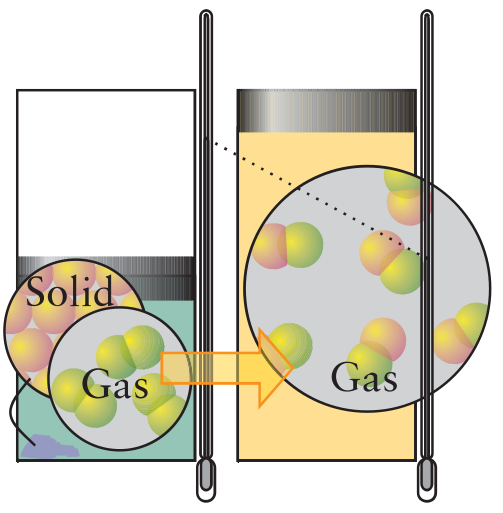
\includegraphics[scale=0.25]{entropy.png}
  b) 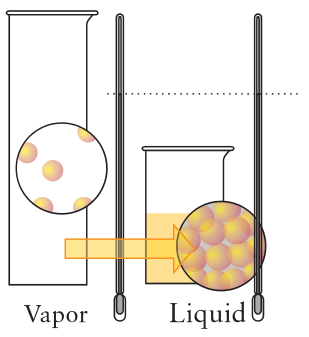
\includegraphics[scale=0.38]{entropy2.png}
\end{center}

\pagebreak

2. (2 pts) \textbf{Equilibrium and Law of Mass Action} Write the equilibrium constant
expression for the following reaction:
\begin{center}
  \ce{NH$_4$HS(s) <=> NH$_3$(g) + H$_2$S(g)}
\end{center}
At 100$^\circ$C, the equilibrium constant is $0.1513$. What is the equilibrium
partial pressure of NH$_3$(g) if the partial pressure of H$_2$S(g) is 4.57 atm. Report
to 3 significant figures.

\vspace{3in}

3. (6 pts) \textbf{Relating Free Energy and Equilibrium Constant} Supposed a reaction
is given by:
\begin{center}
  aA + bB $\rightarrow$ cC + dD
\end{center}
where a, b, ... are the coefficients and A, B, ..., C, D are the reactants and products.

(a) Derive the equation that relates the free energy of reaction ($\Delta G_r$) and the
equilibrium constant $K$ as seen in lecture. Define all variables. \textit{Hint:}
$G(P) = G^\circ + nRT \ln\frac{P}{P^\circ}$.

(b) Using the equation in (a), at what temperature is the following reaction at equilibrium?
\begin{center}
  \ce{CO$_2$(g) + H$_2$O(g) <=> H$_2$(g) + CO$_2$(g)}
\end{center}

% Atkins pg 391

\vspace{3in}

%4. (6 pts) \textbf{Decomposition Reaction}
%
%\begin{center}
%  6 (NH$_4$)$_2$Cr$_2$O$_7$(s) $\rightarrow$ 6 Cr$_2$O$_3$(s) + 4 N$_2$(g) + 6 NH$_3$(g)
%  + 3 O$_2$(g) + 18 H$_2$O(g)
%\end{center}
%
%(a) Balance the chemical reaction.

4. (4 pts) \textbf{Subtitued Benzene} There are three different substituted benzene compounds
with the formula C$_6$H$_4$F$_2$.

(a) Draw the lewis structures of the three compounds.

(b) Assume that the benzene rings pack similarly into their crystal lattices. If the positions
of the H and F atoms are statistically disordered in the solid state, which isomer will have
the \textit{least} molar entropy?

\vspace{3in}

5. (6 pts) \textbf{Air Pollutants} Sulfur trioxide SO$_3$ and nitrogen oxide NO can react in
the atmosphere as follows:
\begin{center}
  SO$_3$(g) + NO(g) $\rightarrow$ SO$_2$(g) + NO(g).
\end{center}
(a) Predict the effect of the following changes to the amount of NO$_2$ when the reacton
has come to equilibrium in a stainless steel bulb equipped with entrants for chemicals
\begin{enumerate}
\item the amount of NO increases
\item the SO$_2$ is removed by condensation
\item the pressure is tripled by pumping in helium
\end{enumerate}

(b) Given that a certan temprature $K = 6.0\times 10^3$, calculate the amount (in moles)
of NO that must be added to a $1.00$ L vesssel containing 0.245 mol SO$_3$(g) to form
0.240 mol SO$_2$(g) at equilibrium. Report to 3 significant figures.

\pagebreak

6. (4 pts) In a sealed 1.75 L vessel at 250$^\circ$C, equilibrium is established between
PCl$_5$(g) and its dissociation products, PCl$_3$(g) and Cl$_2$(g). The quantities found
at equilibrium are 0.562g PCl$_5$, 1.950g PCl$_3$, and 1.007g Cl$_2$. What is the value of
$K_c$ and $K_p$ for the reaction
\begin{center}
  \ce{PCl$_5$(g) <=> PCl$_3$(g) + Cl$_2$(g)}
\end{center}

%\textbf{Ammonia as an Energy Source} Ammonia NH$_3$(g) has been
%investigated as a new energy source for power generators.
%
%(a) Write the balanced chemical equation and equilibrium constants for the combustion of ammonia %at 651C$^\circ$
%and the combustion of gasoline fuel (C$_8$H$_{18}$). %at 370C$^\circ$.
%
% https://doi.org/10.1016/j.applthermaleng.2019.02.072

\vspace{2in}

7. (4 pts) \textit{Extra Credit:} Determine $K_c$ at 300K for the unbalanced equation
\begin{center}
  \ce{CH$_4$(g) <=> C$_2$H$_2$(g) + H$_2$(g)}
\end{center}
Report to 2 significant figures and given the following data
\begin{center}
  \ce{CH$_4$(g) + H$_2$O(g) <=> CO(g) + H$_2$(g) $\,\,$ $K_p = 1.2\times 10^{-25}$}

  \ce{C$_2$H$_2$(g) + O$_2$(g) <=> CO(g) + H$_2$O(g) $\,\,$ $K_p = 1.1\times 10^2$}

  \ce{H$_2$(g) + O$_2$(g) <=> H$_2$O(g) $\,\,$ $K_p = 1.1\times 10^{40}$}
\end{center}

% https://www.chm.uri.edu/weuler/chm112/oldchap14answers.html

\vfill
\textbf{Optional Additional Problems:} Ch. 15 - odd problems 21 - 49 

\end{document}
